
%% add 'handout' option for handouts, and pgfpages for 2-on-1
\documentclass[smaller,compress]{beamer}   
%\usepackage{pgfpages}
%\pgfpagesuselayout{2 on 1}[letterpaper,border shrink=5mm]
%\pgfpagesuselayout{4 on 1}[letterpaper,border shrink=5mm]
%\pgfpagesuselayout{2 on 1}[a4,border shrink=5mm]


\mode<presentation>
{
  %\usetheme[secheader]{Madrid} % nice (once my coloroverrides are sorted out)
  %\usetheme{AnnArbor}	% nice!	
  %\usetheme{Malmoe}	% nice!	
  \usetheme{Warsaw}	% nice!	

  %\usetheme[secheader]{Boadilla} % ok
  %\usecolortheme{whale}
  %\usecolortheme{orchid}
}

% Delete this, if you do not want the table of contents to pop up at
% the beginning of each subsection (or section)
% edd: Does not work in handout mode, and we have too many section/subsections
%\AtBeginSection[]{%
%  \begin{frame}<beamer>%
%    %\tiny
%    \frametitle{Outline}%
%    \tableofcontents[currentsection]%
%  \end{frame}
%}


% If you wish to uncover everything in a step-wise fashion, uncomment the following command: 
%\beamerdefaultoverlayspecification{<+->}

\newcommand{\MedSkip}{\medskip \par} % add \pause if desired 
\newcommand{\SmallSkip}{\smallskip} % add \pause if desired 

\usepackage[english]{babel}   	% or whatever
\usepackage[latin1]{inputenc}	% or whatever
\usepackage{times}
\usepackage[T1]{fontenc}	% Or whatever. Note that the encoding and the 
				% font should match. If T1 does not look
                                % nice, try deleting the line with the fontenc.
%\usepackage{highlight}

\usepackage{listings}
\lstset{ %
  language=R,                   % choose the language of the code
  basicstyle=\scriptsize,       % the size of the fonts that are used for the code
  numbers=left,                 % where to put the line-numbers
  numberstyle=\tiny,            % the size of the fonts that are used for the line-numbers
  stepnumber=1,                 % the step between two line-numbers. If it's 1 each line will be numbered
  numbersep=5pt,                % how far the line-numbers are from the code
  backgroundcolor=\color{white},% choose the background color. You must add \usepackage{color}
  showspaces=false,             % show spaces adding particular underscores
  showstringspaces=false,       % underline spaces within strings
  showtabs=false,               % show tabs within strings adding particular underscores
  frame=single,                 % adds a frame around the code
  tabsize=2,                    % sets default tabsize to 2 spaces
  captionpos=b,                 % sets the caption-position to bottom
  breaklines=true,              % sets automatic line breaking
  breakatwhitespace=false,      % sets if automatic breaks should only happen at whitespace
  escapeinside={\%*}{*)}        % if you want to add a comment within your code
}

\hypersetup{                  		% beamer colors taken from elsewhere
  hyperindex,%				% works with the beetle colour scheme
  colorlinks,%
  linktocpage,%
  plainpages=true,%
  linkcolor=myOrange,%
  citecolor=myDarkGrey,%
  urlcolor=myDarkBlue,%
  pdfstartview=Fit,%
  pdfview={XYZ null null null}%
}
%\hypersetup{                  		% beamer colors taken from elsewhere
%  hyperindex,%				% works with the beetle colour scheme
%  colorlinks%
%  linktocpage,%
%  plainpages=false,%
%  linkcolor=eddBlue,%
%  citecolor=eddDarkGrey,%
%  urlcolor=eddDarkBlue,%
%  pdfstartview=Fit,%
%  pdfview={XYZ null null null}%
%}

\RequirePackage{color}
\definecolor{Red}{rgb}{0.7,0,0}
\definecolor{myOrange}{rgb}{0.8,0.5,0.0}
\definecolor{myBlue}{rgb}{0.0,0.0,0.4}
\definecolor{myDarkBlue}{rgb}{0.1,0.1,0.4}
\definecolor{myDarkGrey}{rgb}{0.15,0.15,0.15}
% Doug's
\definecolor{Sinput}{rgb}{0,0,0.56}
\definecolor{Scode}{rgb}{0,0,0.56}
\definecolor{Soutput}{rgb}{0.56,0,0}
% 
\definecolor{Cmdinput}{rgb}{0,0,0.44}
\definecolor{Cmdoutput}{rgb}{0.44,0,0}
\definecolor{Cppinput}{rgb}{0.15,0.15,0.15}

%% from Doug, but mod'ed \R to use hyperref
\RequirePackage{fancyvrb}
\RequirePackage{xspace}
\RequirePackage{paralist}
\newenvironment{Schunk}{\par\begin{minipage}{\textwidth}}{\end{minipage}}
\DefineVerbatimEnvironment{Sinput}{Verbatim}{formatcom={\color{Sinput}},fontsize=\small}
\DefineVerbatimEnvironment{Soutput}{Verbatim}{formatcom={\color{Soutput}},fontsize=\footnotesize}
\DefineVerbatimEnvironment{Scode}{Verbatim}{formatcom={\color{Scode}},fontsize=\small}
\DefineVerbatimEnvironment{Cmdinput}{Verbatim}{formatcom={\color{Cmdinput}},fontsize=\small}
\DefineVerbatimEnvironment{Cmdoutput}{Verbatim}{formatcom={\color{Cmdoutput}},fontsize=\footnotesize}
\DefineVerbatimEnvironment{Cppinput}{Verbatim}{formatcom={\color{Cppinput}},fontsize=\small}

% -- not \small 
\newcommand{\smallcode}[1]{{\color{Sinput}\small\texttt{#1}}}
\newcommand{\code}[1]{{\color{Sinput}\texttt{#1}}}
\newcommand{\Emph}[1]{\emph{\color{Scode}#1}}   
%\newcommand{\R}{\href{http://www.r-project.org}{\Emph{R}\xspace}}   %% ? sing \emph upsets beamer inside \href
\newcommand{\R}{\href{http://www.r-project.org}{\textsf{R}\xspace}}
\newcommand{\Rns}{\href{http://www.r-project.org}{\textsf{R}}}

% two old defintions
%\newcommand{\code}[1]{\texttt{#1}}
\newcommand{\screenshot}[1]{\centerline{\includegraphics[height=7.8cm,transparent]{#1}}}  % 7.8in


% If you have a file called "university-logo-filename.xxx", where xxx
% is a graphic format that can be processed by latex or pdflatex,
% resp., then you can add a logo as follows:
% NB transparent in Adobe but not in kpdf
\pgfdeclareimage[height=0.6cm]{useR-logo}{figures/useR}
\logo{\pgfuseimage{useR-logo}}


%%% Local Variables: 
%%% mode: latex
%%% TeX-master: "introhighperfR"
%%% End: 
  %% has all definitions etc

%\title[cran2deb: Automated CRAN to Debian packages generation]{cran2deb: A
%  system to automatically provide 1700+ CRAN packages as Debian binaries} 
\title[cran2deb: CRAN to Debian packages]{cran2deb: Automating CRAN to Debian packages generation} 

%\subtitle{\textsl{Tutorial at R/Finance 2009}}
\subject{UseR! 2009 Presentation}
\author[Charles Blundell \and Dirk Eddelbuettel]{Charles Blundell\inst{1} \and Dirk Eddelbuettel\inst{2}}
\institute[Gatsby \and Debian]{\inst{1}Gatsby Computational Neuroscience Unit
  \\ University College London \and \inst{2}Debian / R Projects}
\date[UseR! 2009]{Presentation at UseR! 2009 \\ Rennnes, France \\ July 2009}


\begin{document}

\begin{frame}
  \titlepage
\end{frame}

\begin{frame}
  \frametitle{Overview}
  \tableofcontents
\end{frame}

\section[Why]{Why: Background and Motivation}
\begin{frame}
  \frametitle{About R -- and its repos}
  \framesubtitle{An open statistical language / environment -- with lots of
    excellent code contributions}

  A few key facts that are non-controversial at a \textsl{useR!} conference:
  \begin{itemize} 
  \item \R\ is now a standard for statistical applications and research
  \item \textit{``Success has many fathers''}: several key drivers can
    be identified as to why \R\ has done so well 
  \item We would like to stress \textsl{repos} and available packages here:
    CRAN, as well as BioConductor and Omegahat.
  \item CRAN has been one of the drivers: an open yet rigourously QA'ed
    repostory which has experienced tremendous growth
  \end{itemize}
\end{frame}

\begin{frame}
  \frametitle{CRAN Packages} %% NB Or shall we merge this with the preceding slide?
  \framesubtitle{Exponential Growth}

  \begin{columns}
    \begin{column}{3in}
      \begin{figure}
        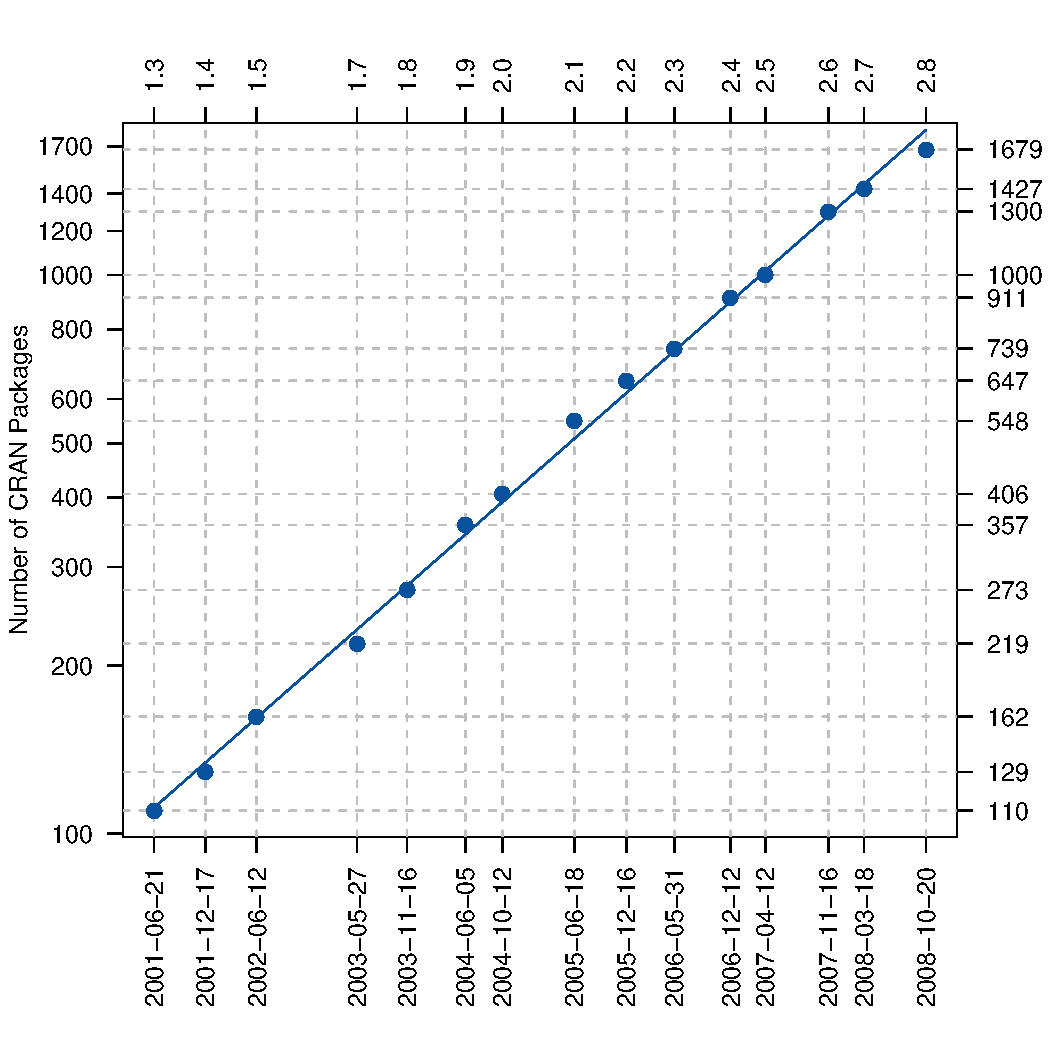
\includegraphics[height=6cm,transparent]{figures/Packages}

        \begin{scriptsize}
          Source: Fox (2008, 2009), our calculations
        \end{scriptsize}
      \end{figure}
    \end{column}
    \begin{column}{2in}
      \begin{itemize} 
        \item CRAN archive network growing by 40\% p.a., now at around 1750 packages

        \item John Fox provided this chart in an invited lecture at the last
        \emph{useR!} meetings.
      \end{itemize}
    \end{column}
    \begin{column}{0.25in}
      \phantom{XX}
    \end{column}
  \end{columns}  
\end{frame}

\begin{frame}
  \frametitle{Debian and Ubuntu} % NB Maybe skip this slide?
  \framesubtitle{Open Linux distributions}

  A few key points:
  \begin{itemize} 
  \item Debian is \textsl{the} community-driven Linux distribution where
    numerous volunteers provide over twenty-thousand packages for around
    a dozen architectures.
  \item Packages and package management ``just work'': with arguably the most
    advanced and robust package management system, and a tremendous
    build and test infrastructure.
  \item Ubuntu has taken Debian, added a fair amount of spit and polish, as
    well as regular bi-annual releases, and has rapidly gained mind- and
    well as market-share as the Linux distribution to beat.
  \item Lastly, we note that the CRAN backend is also implemented on Debian.
  \end{itemize}
\end{frame}

\begin{frame}
  \frametitle{Why build Debian R packages?}
  \framesubtitle{Combining R and Debian}
  Bates, Eddelbuettel and Gebhard (UseR! 2004) listed a number of reason
  that still hold:
  \begin{itemize} 
  \item \textbf{Dependencies} are resolved automatically: \textsl{it just
      works}
  \item \textbf{Convenience} of installing binary packages via
    \texttt{apt-get} %is
    %easier than building from source
  \item \textbf{Quality control} as build daemons, automated rebuilds,
    porting, ... all ensure that everything is pretty much buildable all the
    time
  \item \textbf{Scalability} as building one binary package and scripting
    installation on a cluster beats doing lots of manual installations
  \item \textbf{Common platform} as Debian forms the base for Ubuntu and
    several other derivative or single-focus distributions
  \item \textbf{Different architectures} ranging from small arm or mips based
    systems to amd64, sparc64, hppa or even s390 mainframes
  \item \textbf{Audience} given the reach of Debian and Ubuntu, large number
    of users can be reached with little effort
  \end{itemize}

\end{frame}

%\section{What is behind it?}
\begin{frame}
  \frametitle{So what is a Debian package?} % NB Maybe skip this?
  \framesubtitle{And how do I build it?}

  Building a Debian package is similar to using \texttt{R
    CMD binary} etc:
  \begin{itemize} 
  \item Reads meta-information is read from the files in the debian/ directory
    \begin{itemize} 
    \item debian/control (similar to R's DESCRIPTION) lists names,
      maintainers, build- and run-time dependencies
    \item debian/copyright lists all author, license holders and copyright
      statements 
    \item debian/changelog provides current and past version numbers with a
      list of  all changes in chronological fashion
    \item debian/rules is a Makefile containing all steps to configure,
      build, install, package-create and clean
    \end{itemize}
  \item Employs a number of external scripts and tools tie into this,
  similar to what R has below \texttt{\$RHOME/share}
  \end{itemize}
\end{frame}


\section[How]{How: Key aspects of the approach and implementation}
\begin{frame}
  \frametitle{Comparing two approaches}
  \framesubtitle{What have we learned?}

  Eddelbuettel, Vernazobres, Gebhard and M\"{o}ller (UseR 2007) presented a first
  approach.

  \MedSkip

  \begin{columns}
    \begin{column}{2in}
      \textsl{Then}
      \begin{itemize}
      \item Top-down approach 
      \item Monolithic and large Perl program 
      \item Re-implementing chunks of what \R does in parsing archives
      \item Not very robust
      \end{itemize}
    \end{column}      

    \begin{column}{2in}
      \textsl{Now}
      \begin{itemize}
      \item Bottom-up approach
      \item Collection of \R and shell scripts, also lots of SQL
      \item Re-using \R internal infrastructure as much as possible
      \item Influenced by %Eddelbuettel's
        \href{http://dirk.eddelbuettel.com/cranberries/}{CRANberries} and its
        200 lines of \R code to monitor and summarize CRAN changes
      \end{itemize}
    \end{column}      
  \end{columns}
\end{frame}

\begin{frame}
  \frametitle{Technology Overview}
  \framesubtitle{Charles: Can you fill something in here, if I haven't stolen
    all nuggets on the previous slide?}

\end{frame}

\section[Status]{Status: Where are we now?}
\begin{frame}
  \frametitle{Current Status}
  \framesubtitle{Ready for wider deployment and testing}

  \begin{itemize}
  \item Ground-work provided during Google Summer of Code 2008 under the
    umbrella of the \R Foundation
  \item Currently using a (small) Xen-instance on a server at WU Wien to host
    two Debian pbuilder chroots and an archive
  \item 1700+ packages for i386 and amd64 on Debian testing
  \item In daily use for the last few weeks!
  \end{itemize}

  \MedSkip
  Just add the following URL (with -amd64 for 64-bit) \newline 
  { \SmallSkip \scriptsize
    \texttt{deb http://xmcorsairs.wu.ac.at/cran2deb/debian-i386 testing/}
  }

\end{frame}

\section{Open Issues}
\begin{frame}
  \frametitle{Question to be addressed}
  \framesubtitle{These may not be showstoppers}

  \begin{itemize}
  \item What can or cannot be (re-)distributed by CRAN and its mirrors?
  \item What can or cannot be used by all users?
  \item Remaining external dependencies: 
    \begin{itemize}
      \item BioConductor is the single largest source: BioBase, RGraphviz, etc
      \item Other external libraries or tools not in Debian 
      \item Commercial external dependencies: SGE, LSF, Oracle, Vhayu
    \end{itemize}
  \item Builds for other architectures ?
  \item Builds for other Debian flavours such as Ubuntu ?
  \end{itemize}
\end{frame}

\end{document}

%%% Local Variables: 
%%% mode: latex
%%% TeX-master: t
%%% End: 
